\chapter{Magmatisme intrusif}
\label{chap1}
\minitoc

\section{Formation, transport et stockage des magmas}
\label{C1-sec:magm-intr-un}

\subsection{Formation}
\label{C1-sec:formation-1}

La majorité des magmas sont formés  par fusion partielle des roches du
manteau  supérieur.   Dans les  conditions  normales  de pression,  la
température du  manteau supérieur  n'est pourtant pas  suffisante pour
provoquer leur  fusion (Figure \ref{C1-Geoterme}) et  d'autres mécanismes
sont  nécessaires pour  amener les  roches du  manteau à  croiser leur
liquidus.  Au niveau  des dorsales en contexte océanique  ou des rifts
en contexte continental  ou encore au sein  des panaches mantelliques,
la  fusion  partielle  est  ainsi  générée  par  décompression  (Figure
\ref{C1-Geoterme} b).  Au niveau des  zones de subduction, les mécanismes
mis en jeu  sont plus complexes et font  intervenir la déshydratation
par chauffage des roches et la migration des fluides abaissant le
liquidus, provoquant ainsi la fusion des roches alentour (Figure
\ref{C1-Geoterme} c).

\begin{figure}[htpb]
  \begin{center}
    \graphicspath{ {/Users/thorey/Documents/These/Manuscript/Figure/Chapter1/} }
    \includegraphics[scale=1.3]{Temperature-Profile.eps}
    \caption{a) Lien entre le magmatisme et la tectonique des plaques:
      production de  magma par  fusion partielle par  décompression au
      niveau  des  dorsales  océaniques   ou  des  rifts  en  contexte
      continental ou par addition de  volatiles au niveau des zones de
      subduction. Schéma du  diagramme de phase des  roches du manteau
      supérieur dans  deux contextes différents: b)  dorsale océanique
      ou panache mantellique, c) zone de subduction.}
    \label{C1-Geoterme}
  \end{center}
\end{figure}

\subsection{Transport}
\label{C1-sec:transport}

Les liquides de fusions ainsi formés  sont moins denses que les roches
solides alentour et  s'élèvent donc, par compaction  et percolation au
travers          de           la          matrice          mantellique
\citep{McKenzy:1984bo,McKenzie:1985jq}. Le magma, liquide de fusion et
cristaux, s'accumule ensuite au sein de  chenaux, i.e.  de dykes ou le
long de faille préexistantes pour remonter rapidement vers les couches
superficielles               de                la               croûte
\citep{Lister:1991ut,Clemens:1992kr,Petford:1993bk,Rubin:1995upa}.  En
effet, bien  que l'idée du magma  remontant lentement au sein  de gros
volumes diapiriques  soit encore parfois  invoquée au sein de  la base
ductile  de  la   croûte  \citep{Weinberg:1994jg,Weinberg:1996vb},  le
transport rapide  du magma  au sein  des dykes  permet de  résoudre de
nombreux problèmes,  thermiques et  mécaniques, associés à  la remonté
diapirique de  gros volume  de magma au  sein des  parties supérieures
fragiles de la croûte invoquée historiquement \citep{Miller:1999km}.

\subsection{Stockage}
\label{C1-sec:stockage}

Les  travaux  de  \citet{Walker:1989jq}  ont  montré  que  les  magmas
remontent  jusqu'à rencontrer  leur zone  de flottabilité  neutre, une
région où  la densité de la  roche encaissante est proche  de celle du
magma lui-même. En effet, au-dessus de cette couche, le magma est plus
dense que la  roche encaissante et sa flottabilité  l'entraîne vers le
bas.        De      nombreux       travaux,      tant       théoriques
\citep{Lister:1991ut,Petford:1993bk,Rubin:1995upa}    qu'expérimentaux
\citep{Taisne:2009kj,Taisne:2011do}  ont en  effet  depuis montré  que
l'ascension d'un  dyke était  contrôlée par  la différence  de densité
entre la  tête de celui-ci  et la  roche encaissante. Lorsque  le dyke
entre dans  une région de  densité inférieure, la  surpression induite
peut, sous  certaines conditions, conduire  à l'étalement du  magma au
niveau de la base de la  région de plus forte densité permettant ainsi
ainsi  la formation  de  réservoir magmatique  sous forme  d'intrusion
magmatique au sein de la croûte \citep{Taisne:2011do}.

Plus  récemment, d'autres  études  ont montré  que  les contrastes  de
rigidité  entre les  différentes  couches  crustales pourraient  aussi
jouer un  rôle non  négligeable sur l'arrêt  de l'ascension  des dykes
\citep{Menand:2011ki}.   En  effet,   des  expériences  réalisées  par
\citet{Kavanagh:2006ig} ont  montré que la propagation  d'un dyke peut
être  arrêtée quand  celui-ci rencontre  une interface  qui sépare  un
milieu  plus  rigide  surplombant   un  milieu  moins  rigide  (Figure
\ref{C1-Neutral_Zone}). Le  dyke arrête ainsi son  ascension verticale
et s'étale horizontalement  juste en dessous de la  couche de rigidité
plus  élevée.   Ce mécanisme  serait  d'autant  plus efficace  que  le
contraste de rigidité est important \citep{Kavanagh:2006ig}.

\begin{figure}[htpb]
  \begin{center}
    \graphicspath{ {/Users/thorey/Documents/These/Manuscript/Figure/Chapter1/} }
    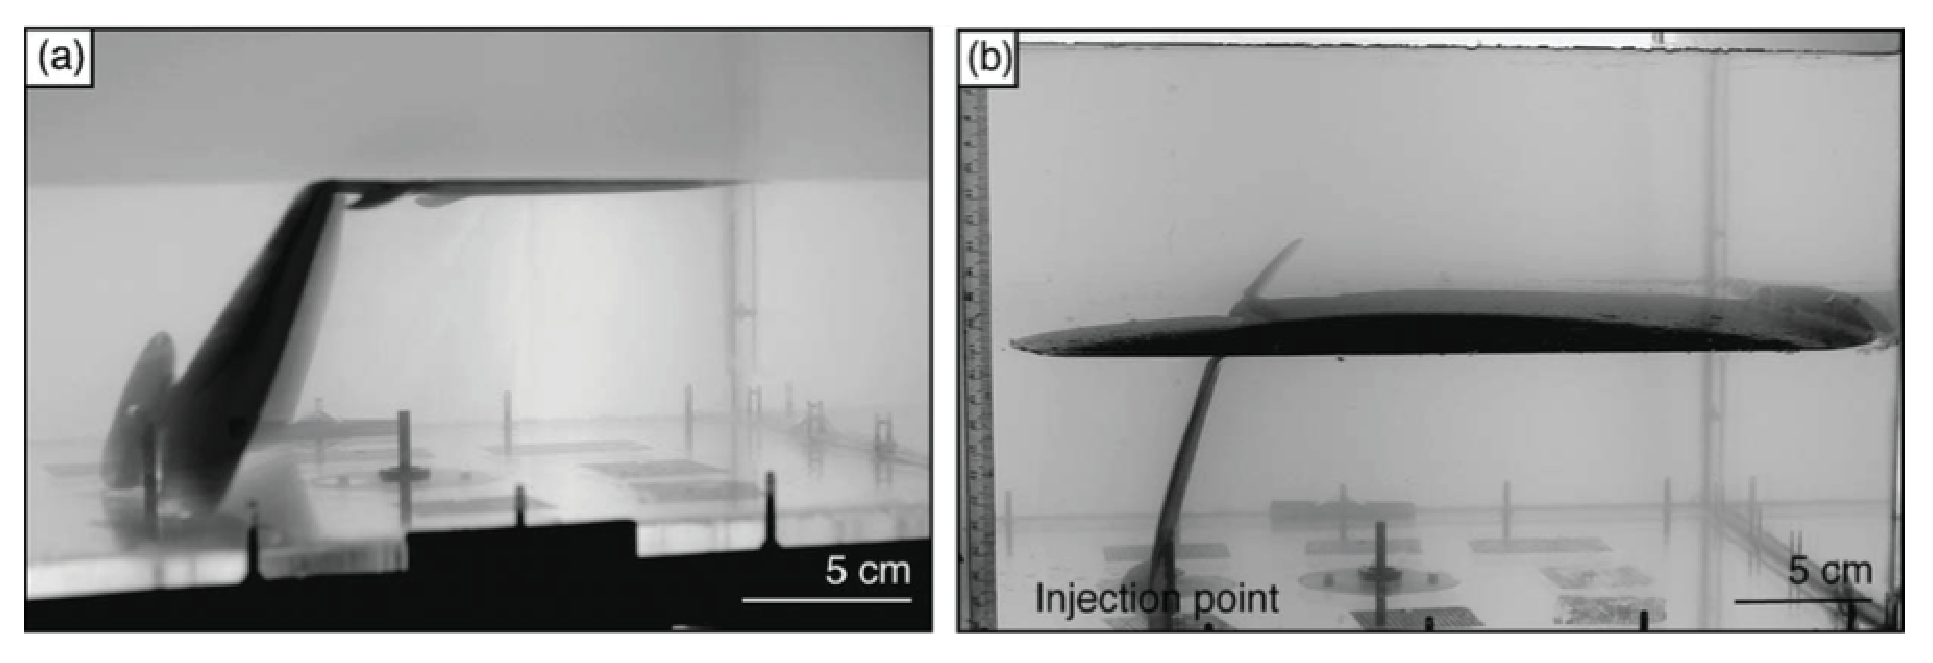
\includegraphics[scale=0.4]{Neutral_Zone.eps}
    \caption{a)  Photographie de  deux des  expériences réalisées  par
      \citet{Kavanagh:2006ig}   sur  le   comportement  d'un   dyke  à
      l'interface  entre deux  milieux de  rigidité différente.  a) Le
      contraste de rigidité est très important et le dyke s'étale sous
      la couche de  rigidité importante.  b) Le  contraste de rigidité
      est plus faible et, tout en s'étalant en dessous de la couche de
      rigidité  supérieure, le  dyke continue  sa progression  dans le
      milieu plus rigide.}
    \label{C1-Neutral_Zone}
  \end{center}
\end{figure}


Finalement, les contraintes, locales ou globales, peuvent aussi dévier
la trajectoire d'un dyke et influencer  les trajets des magmas au sein
de la  croûte.  En effet,  des études ont  montré que les  chenaux par
lesquels se propage le  magma tendent à s'orienter perpendiculairement
aux contraintes  de compression \citep{Anderson:L5JA3dNN}.   Les dykes
ont donc  tendance à exister  dans des situations dans  lesquelles les
contraintes de compressions sont horizontales et donc à s'étaler quand
le  champ  de  contrainte   évolue  d'une  contrainte  de  compression
horizontale à  vertical comme c'est le  cas par exemple au  niveau des
édifices volcaniques \citep{Pinel:2000wa,Pinel:2004ji,Roman:2014hw}.

Cependant, si ces  différents facteurs jouent un rôle  sur le contrôle
des trajets  des magmas au sein  de la croûte, la  densité relative du
magma et  de la  roche encaissant  et donc  l'existence d'une  zone de
flottabilité neutre  est certainement  le facteur le  plus déterminant
dans  la  mise  en  place  d'intrusions  magmatiques.   Le  magmatisme
intrusif, et  donc la  question du  stockage des  magmas, est  donc de
manière  générale étroitement  lié à  la  structure en  densité de  la
crôute elle-même.


\section{Importance et multiples visages du magmatisme intrusif}
\label{C1-sec:zool-des-intr}

\subsection{Magmatisme intrusif sur Terre}
\label{C1-sec:definition}

Sur  Terre, la  composition  de la  croûte, et  donc  sa densité,  est
bimodale.   Au niveau  des océans,  la croûte  océanique présente  une
nature essentiellement  basaltique avec une densité  moyenne proche de
$2900$ kg  m$^{-3}$.  Elle  est formée  continuellement au  niveau des
dorsales océaniques et recyclée, environ $200$ Ma d'année plus tard au
niveau des zones de subduction. Elle  est épaisse en moyenne de $6$ km
et couvre à elle seule $70\%$ de la surface du globe. Au contraire, la
croûte  continentale, qui  occupe  les $30\%$  restants, présente  une
composition plus  évoluée et globalement andésitique  avec une densité
moyenne plus  proche de  $2700$ kg m$^{-3}$.   Elle est  beaucoup plus
vieille que  la croûte océanique et  est âgée en moyenne  de $2.5$ Ga,
avec certaines roches ayant été  datées jusqu'à $4$ Ga d'années.  Elle
est  aussi  beaucoup plus  épaisse  que  la croûte  continentale;  son
épaisseur moyenne est  de $35$ km et peut excéder  les $70$ kilomètres
sous certaines chaînes de montagnes comme l'Himalaya.

De par  sa densité  relativement basse, en  particulier au  niveau des
continents, la croûte  constitue un filtre efficace à  la remontée des
magmas  en  surface  qui   sont  donc  préférentiellement  stockés  en
profondeur sous forme  d'intrusions magmatiques.  \citet{Crisp:1984dm}
et  \citet{White:2006gr} estiment  en effet  que les  volumes de  lave
extrudée à  la surface  sont relativement  faibles en  comparaison des
volumes mis  en place au sein  de la croûte terrestre,  i.e.  $5$ fois
plus faibles en  contexte océanique et jusqu'à $10$  fois plus faibles
en contexte  continental.  Le magmatisme intrusif  apparaît donc comme
un processus essentiel dans la formation de la croûte.  Sur Terre, les
mouvements  tectoniques en  son sein  ainsi que  l'érosion ont  permis
d'exposer  certaines  de ces  intrusions  à  la surface.   Outre  leur
taille,  qui  peut  varier  de  quelques mètres  à  des  centaines  de
kilomètres,  la  morphologie de  ces  intrusions  présente une  grande
variabilité.

Les batholites sont de loin  les plus imposants représentants de cette
famille d'intrusions  magmatiques se  mettant en place  au sein  de la
partie fragile de  la croûte.  Ils peuvent  atteindre jusqu'à quelques
kilomètres d'épaisseur  et s'étendre sur des  centaines de kilomètres.
Par  exemple,  le  batholite  de   Sierra  Nevada  est  une  intrusion
granitique qui s'étend sur presque la  totalité de la Sierra Nevada en
Californie.   Des   données  géochronologiques  sur  certain   de  ces
batholites ont  montré que  leur mise en  place peut  s'échelonner sur
quelques millions d'années, un temps beaucoup plus grand que les temps
raisonnables pour le refroidissement  d'une chambre magmatique dans la
partie fragile de  la croûte \citep{Glazner:2004gv}. En  effet, il est
maintenant clair que  la mise en place de ces  gigantesques volumes de
magmas se fait par incréments successifs de petits volumes de magma se
solidifiant lors  de leur  mise en  place sur  de longues  échelles de
temps,         de        $10^5$         à        $10^6$         années
\citep{Petford:2000cc,Glazner:2004gv}.   Dans cette  thèse, nous  nous
focalisons donc sur les mécanismes de formation et de mise en place de
volumes intermédiaires  de magma dans  la partie fragile de  la croûte
continentale, à des profondeurs inférieures à $10$ km.

Des études  géologiques de  terrain ont montré  la présence  de quatre
grandes familles  d'intrusions magmatiques  de taille  intermédiaire à
faible profondeur.  Deux de ces familles, les dykes et les bysmalites,
sont  discordantes,   c'est-à-dire  qu'elles   se  mettent   en  place
perpendiculairement à  la stratification naturelle de  l'encaissant et
deux  autres,   les  sills  et  les   laccolites,  sont  concordantes,
i.e. elles se mettent en place parallèlement aux couches géologiques.

\begin{figure}[htpb]
  \begin{center}
    \graphicspath{ {/Users/thorey/Documents/These/Manuscript/Figure/Chapter1/} }
    \includegraphics[scale=0.5]{Intrusive_Activity.eps}
    \caption{a) Différentes formes  du magmatisme intrusif: batholite,
      dyke,  sill   et  laccolite.    Dimensions  typiques   pour  des
      laccolites,   dyke  et   sill  de   composition  et   d'origines
      différentes repris de \citet{Cruden:tg}. }
    \label{C1-Dimension}
  \end{center}
\end{figure}

\begin{itemize}
\item  Les  dykes,  par  lesquels  remontent le  magma  à  travers  la
  lithosphère sont discordants et caractérisés par de faibles rapports
  d'aspects  (Figure  \ref{C1-Dimension}, \ref{C1-picture}  a).   Leur
  épaisseur peut  varier de  quelques mètres  à quelques  centaines de
  mètres  d'épaisseur \citep{Walker:1989jq,Rubin:1995upa},  cependant,
  l'épaisseur moyenne est de quelques dizaines de mètres. Les dykes de
  compositions felsiques  sont généralement plus épais  et moins longs
  que leurs équivalents mafiques \citep{Rubin:1995upa}.

\item Les sills,  à la différence des dykes,  sont concordants (Figure
  \ref{C1-Dimension}, \ref{C1-picture} b,f).  Ils  se mettent en place
  le long de discontinuités ou de failles préexistantes, à la jonction
  entre  deux  couches  sédimentaires  par  exemple.   Les  sills  aux
  dimensions les plus importantes répertoriés sont mafiques et peuvent
  attendre  jusqu'à $100$  km sur  des  épaisseurs de  presque $1$  km
  \citep{Cruden:tg}.   Leurs homologues  felsiques,  plus rares,  sont
  souvent de dimension plus faible.

  \begin{figure}[htpb]
    \begin{center}
      \graphicspath{ {/Users/thorey/Documents/These/Manuscript/Figure/Chapter1/} }
      \includegraphics[scale=0.95]{photo.eps}
      \caption{a) Dyke  traversant des  couches sédimentaires  dans le
        Makhtesh  Ramon,  Israël;  b)   Sill  basaltique  au  sein  de
        sédiments, vallée  de la  Yellowstone River, parc  National du
        Yellowstone  (USA).   Photographie  de  Fabrice  Pinchon.   c)
        Laccolite   à  l'érosion   dans  le   Montana  d)   Schéma  de
        l'emplacement       d'un      laccolite       réalisé      par
        \citet{Gilbert:1877uk}. e) Schéma simplifié de la structure en
        arbre de noel d'un complexe  de laccolite sur l'île d'Elbe, en
        Italie,  étudiée par  \citet{Rocchi:2010dn}.  f)  Intrusions à
        l'érosion au alentour  de la montagne Hillers,  dans les Henry
        Mountains.   On peut  distinguer  le Black  Mesa Bysmalite  au
        centre et  le Maiden Creek  sill en dessous.   Photographie de
        Jack Share}
      \label{C1-picture}
    \end{center}
  \end{figure}

\item    Les   laccolites    ont   été    décrit   premièrement    par
  \citet{Gilbert:1877uk}  suite  à  son  étude  géologique  des  Henry
  Mountains, dans l'Utah aux États-Unis (Figure \ref{C1-picture} c, d,
  e).  Ils se mettent en  place principalement par flexion des couches
  sédimentaires  sus-jacentes, ce  qui leur  donne une  forme de  dôme
  caractéristique.    Certains   d'entre   eux  peuvent   aussi   être
  caractérisés  par   une  forme  un   peu  plus  aplatie   au  centre
  \citep{Koch:1981if}. \citet{E:2015tl} a répertorié  à peu près $900$
  laccolites,  principalement  dans  le nord  des  États-Unis.   Leurs
  épaisseurs  varient de  quelques  dizaines à  quelques centaines  de
  mètres et  leurs rayons  peuvent atteindre quelques  kilomètres pour
  les plus gros (Figure \ref{C1-Dimension} b).  Ces laccolites se sont
  parfois mis en place les uns sur les autres formant une structure en
  forme de sapin de Noël  \citep{E:2015tl}.  Cette géométrie est aussi
  observée  sur  l'île d'Elbe,  en  Italie,  où  un complexe  de  neuf
  laccolites, exceptionnellement bien conservé, a été étudié en détail
  par \citet{Rocchi:2002jy}.

\item   Les   bysmalites   sont  d'imposants   volumes   cylindriques,
  préférentiellement composés de roche granitique, discordants (Figure
  \ref{C1-picture} f).   Ils sont  notamment bordés  par d'importantes
  failles presque  verticales et peuvent atteindre  quelques centaines
  de mètres d'épaisseur \citep{Johnson:1973ho}.  Un exemple typique de
  ce  type d'intrusion  est le  Black  Mesa Bysmalite  dans les  Henry
  Mountains   ($200$    m   d'épaisseur    et   $1$   km    de   large
  \citep{Morgan:2008hj}).
\end{itemize}

À  l'instar des  batholites,  de nombreuses  observations de  terrains
proposent que  ces intrusions de  taille moyenne se forment  aussi par
incréments     successifs    de     petits     volumes    de     magma
\citep{Habert:2004wg,Horsman:2005ct,Morgan:2008hj}             (Figure
\ref{C1-Horsmann}).  Cependant,  les mêmes  études montrent  aussi que
ces intrusions  se forment nécessairement  sur de petites  échelles de
temps, des échelles  assez faibles pour pouvoir garder  un corps chaud
et  liquide  des  premières  étapes  du  processus  d'intrusion  à  la
solidification.   Au niveau  du bysmalite  de Black  Mesa par  exemple
(Figure   \ref{C1-picture}   f),  \citet{Habert:2004wg}   ont   montré
l'absence de  discontinuités entre  les différentes couches  ainsi que
l'absence de  métamorphisme important  dans l'encaissant  indiquant un
temps  de  mise  en  place  de  moins  de  $100$  ans.   L'absence  de
discontinuité  au  sein des  différents  laccolites  sur l'île  d'Elbe
supporte aussi  leur formation  rapide, i.e.  à  la suite  d'une seule
injection où de plusieurs injections sur un temps assez court pour que
les magmas des différentes injections coalescent \citep{Roni:2014gt}.

\begin{figure}[htpb]
  \begin{center}
    \graphicspath{ {/Users/thorey/Documents/These/Manuscript/Figure/Chapter1/} }
    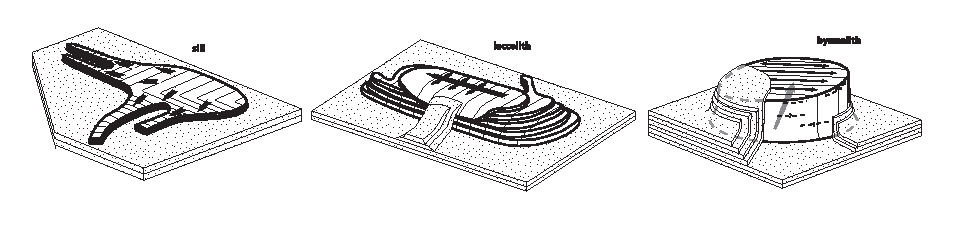
\includegraphics[scale=0.8]{Horsmann.eps}
    \caption{Ces  diagrammes,  réalisés  par  \citet{Horsman:2009gea},
      montrent la structure verticale en  couche de trois intrusions à
      l'érosion  dans les  Henry  Mountains. De  gauche  à droite:  le
      Maiden Creek Sill (Figure  \ref{C1-picture} f), le Trachyte Mesa
      Laccolite et  le Black  Mesa Bysmalite  (Figure \ref{C1-picture}
      f).}
    \label{C1-Horsmann}
  \end{center}
\end{figure}

\subsection{Magmatisme intrusif sur la Lune}
\label{C1-sec:moon}

La lune  s'est probablement formée suite  à l'impact d'un corps  de la
taille  de Mars  sur  la proto-Terre  quelques  centaines de  millions
d'années après la  formation de la Terre, le disque  de débris produit
se  réaccrétant ensuite  en moins  d'un millier  d'années pour  former
notre                                                        satellite
\citep{Mizutani:1972hc,Cameron:1991vu,Canup:2001eb,Canup:2012cd}.
Compte  tenu des  quantités  importantes d'énergie  libérée durant  le
processus  d'accrétion, on  considère  aujourd'hui que  la Lune  était
partiellement fondue,  sur une épaisseur  encore débattue, suite  à sa
formation \citep{ElkinsTanton:2011ce}.  Le refroidissement et la lente
cristallisation fractionnée de l'océan de magma lunaire aurait ensuite
conduit  à  la formation  d'une  croûte  primaire par  flottaison  des
minéraux  légers  de plagioclase  (en  particulier  du pôle  calcique,
l'anorthite) à la surface de l'océan  de magma tandis que les éléments
les  plus incompatibles,  en particulier  les éléments  producteurs de
chaleur, se seraient concentrés dans les derniers liquides magmatiques
résiduels entre la croûte et le manteau, formé, lui, principalement de
cumulats d'olivine et de pyroxène (Figure \ref{C1-MO}).

\begin{figure}[htpb]
  \begin{center}
    \graphicspath{ {/Users/thorey/Documents/These/Manuscript/Figure/Chapter1/} }
    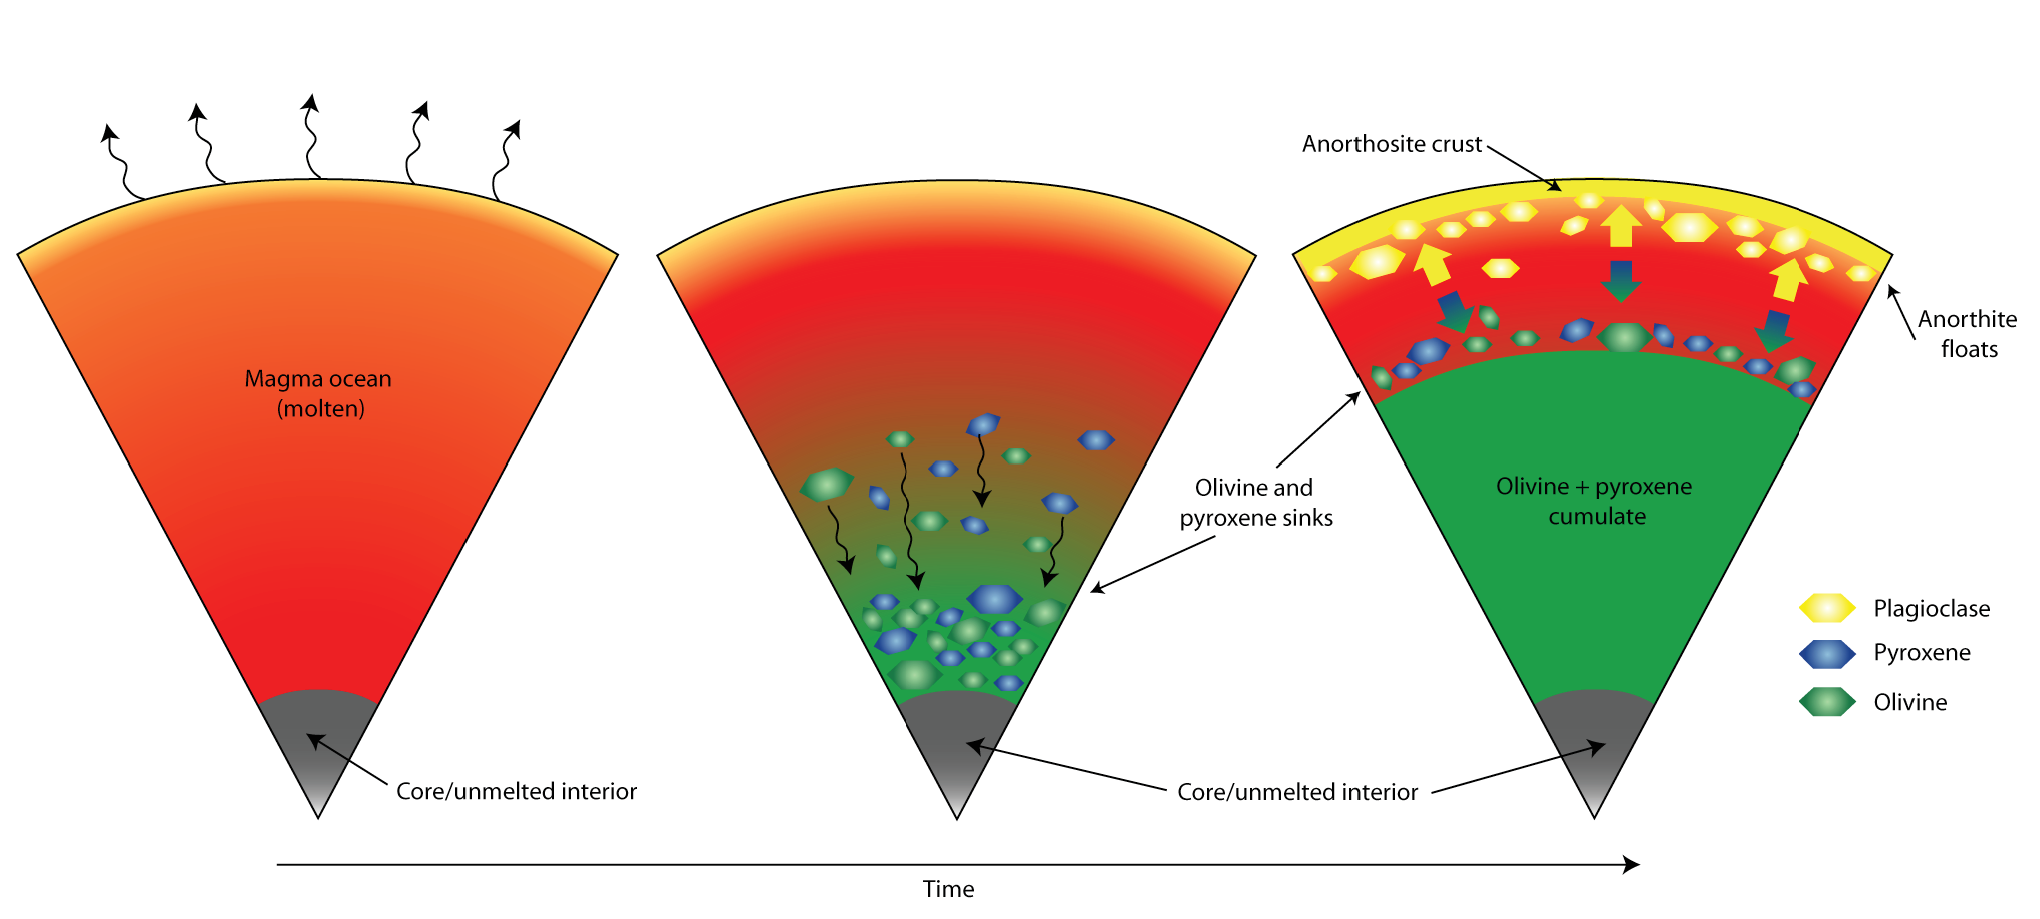
\includegraphics[scale=0.4]{MO.eps}
    \caption{Cristallisation  fractionnée  de   l'océan  de  magma  et
      formation de  la croûte primaire composé  d'anorthosite. Source:
      LPI}
    \label{C1-MO}
  \end{center}
\end{figure}

Etant donné sa composition et  la porosité résultante de $4$ milliards
d'années  de  bombardement  météoritiques,  la densité  de  la  croûte
lunaire  est particulièrement  faible \citep{Huang:2012gf,Han:2014ic}.
D'après les dernières estimations, rendues possibles grâce aux mesures
du champ  de gravité d'une  résolution sans précédent obtenues  par la
mission GRAIL  de la  NASA, la  densité moyenne  au niveau  des terres
hautes serait  de $2550$  kg m$^{-3}$  \citep{Wieczorek:2013ipa}.  Ces
données ont  aussi permis de réévaluer  à la baisse l'épaisseur  de la
crôute à  entre $34$ et  $44$ km en moyenne  avec une tendance  à être
moins épaisse au niveau des mers lunaires.

La faible  densité de sa crôute  et son épaisseur non  négligeable ont
certainement joué  un rôle  important sur  le volcanisme  lunaire.  En
effet,  les  magmas  formées  par   fusion  du  manteau  lunaire  sont
particulièrement   dense,   de   l'ordre   de   $3000$   kg   m$^{-3}$
\citep{Kiefer:2012kp} en  lien avec leur composition  basaltique riche
en oxydes  métalliques, en  particulier en  oxyde de  Fer $FeO$  et de
Titane $T_iO_2$. Ainsi, la  croûte primaire formée par cristallisation
de l'océan de  magma étant très légère, elle a  sans aucun doute aussi
été  un filtre  puissant à  l'éruption des  magmas sur  la lune,  leur
flottabilité  ne  leur permettant  pas  d'être  transporté jusqu'à  la
surface.

\citet{Wieczorek:2001jt}  ont ainsi  confirmé que  le volcanisme  à la
surface  est généralement  lié à  l'extraction d'une  partie de  cette
crôute de  faible densité,  comme c'est  la cas  par exemple  des mers
lunaires  qui  se sont  mises  en  place  au  sein de  larges  bassins
d'impacts. \citet{Head:1992bk} ont estimé  à $50$ fois plus importants
les  volumes de  magma  mis en  place en  profondeur  que les  volumes
éruptés en  surface. Cependant, bien  que ce rapport puisse  donner de
précieuses indications  sur l'évolution thermique et  magmatique de la
lune elle-même, il est de fait très peu contraint et la part intrusive
du  magmatisme  lunaire  est  encore mal  connue.   La  détection  des
déformations de  surface induites  par la  mise en  place d'intrusions
magmatiques  au sein  de la  croûte apparaît  donc comme  une première
étape  visant à  la  meilleur caractérisation  du magmatisme  intrusif
lunaire.

Deux  manifestations principales  à  la  surface de  la  lune ont  été
proposées  comme  potentiellement  résultantes  de la  mise  en  place
d'intrusions magmatiques  au sein  de la croûte  lunaire: les  dômes à
faible pente et les cratères à sol fracturé.

\begin{itemize}
\item Les dômes  à faible pente sont localisés en  bordure ou dans les
  mers   lunaires,  principalement   sur  la   face  visible   (Figure
  \ref{C1-Moon-magma} a, b).  Une quinzaine de ces dômes, possiblement
  d'origine    intrusive,    ont     été    récemment    décrit    par
  \citet{Wohler:2007it}.  Bien que leur  morphologie s'apparente à des
  laccolites terrestres,  ils sont  de manière générale  beaucoup plus
  étalés que  ceux sur  Terre; pour  une même  épaisseur, l'équivalent
  lunaire  peut ainsi  être deux  fois  plus large  que son  homologue
  terrestre.

  \begin{figure}[htpb]
    \begin{center}
      \graphicspath{ {/Users/thorey/Documents/These/Manuscript/Figure/Chapter1/} }
      \includegraphics[scale=0.95]{Moon_Lacc.eps}
      \caption{a)  Dome lunaire,  photo  par Appolo  17  b) Apollo  15
        orbital image  AS15-91-12372, vue  oblique du  dôme Valentine.
        c) Cratère au sol fracture Atlas (Classe 1). d) Cratère au sol
        fracturé  Lavoisier (Classe  5).  e)  Cratère au  sol fracturé
        Gassendi  (Classe  3).  f)  Cratère  au  sol fracturé  Komarov
        (Classe   5).   Photo   extraite   de  \textit{Lunar   Orbiter
          Photographic Atlas of the Moon, NASA}}
      \label{C1-Moon-magma}
    \end{center}
  \end{figure}

\item Les  cratères à sol  fracturé sont des cratères  d'impacts ayant
  subi des déformations suite à leur  formation.  À peu près $ 200$ de
  ces   cratères  ont   été  répertorié   par  \citet{Schultz:1976kt},
  principalement autour des  mers lunaires (Figure \ref{C1-Moon-magma}
  c, d, e, f).  La principale caractéristique de ces cratères est leur
  faible profondeur  par rapport à  celles des cratères  non déformés.
  En effet, certains cratères au sol fracturé peuvent être jusqu'à $2$
  km moins profonds que leurs homologues non déformés.  Leur sol, soit
  en  forme de  dôme, soit  plat séparé  des bords  du cratère  par un
  imposant  fossé  circulaire,  est systématiquement  caractérisé  par
  d'importants réseaux de fractures  radiales, concentriques ou encore
  pentagonales (Figure \ref{C1-Moon-magma} c, d, e, f).  Basé sur leur
  profondeur,     topographie     et    niveau     de     déformation,
  \citet{Schultz:1976kt} a postulé l'existence  de six grandes classes
  de  déformation.   La  proximité  de  ces  cratères  avec  les  mers
  lunaires, ainsi que  la présence de produits volcaniques  au sein de
  certains d'entre  eux, suggère  qu'ils ont été  déformés suite  à la
  mise en place de magma en profondeur sous leur sol.
\end{itemize}

\section{Caractérisation  de   la  mise  en  place   d'une  intrusion
  magmatique à faible profondeur}
\label{C1-sec:orign-theor-fram}

\subsection{Model statique de déformation d'une couche élastique}
\label{C1-sec:model-statique-de}

Bien  que  la  morphologie  et  les volumes  de  magma  puissent  être
récupérés,  à  partir  d'observations   directes  ou  de  méthodes  de
prospection géophysique sur  Terre ou via les  déformations induites à
la  surface  des autres  corps  telluriques  du système  solaire,  ces
informations  seules   ne  donnent  que  peu   d'indications  sur  les
mécanismes  de  mise  en  place de  ces  intrusions  magmatiques.   De
nombreux  travaux  ont  ainsi  été centrés  sur  la  modélisation  des
processus  donnant lieu  à  ces  déformations, dans  le  but de  mieux
comprendre le mécanisme d'intrusion d'une part, mais aussi, de déduire
des  observations  des  informations  sur  le  magma,  les  paramètres
mécaniques de l'encaissant  ou encore la profondeur  de l'intrusion au
moment de sa mise en place.

La  propagation d'un  dyke dans  un  milieu élastique  a été  beaucoup
étudiée    \citep{Lister:1991ut,Rubin:1995upa}.     En    particulier,
\citet{Lister:1991ut} ont montré que, à l'exception de la tête du dyke
où  les contraintes  élastiques induites  par les  roches encaissantes
jouent un  rôle important, la dynamique  du magma au sein  du dyke est
contrôlée  par un  équilibre entre  la flottabilité  et les  pertes de
charge associées aux  frottements visqueux sur les  parois du conduit.
On a vu  qu'un dyke peut se transformer en  sill si celui-ci rencontre
sa zone de flottabilité neutre; bien que la dynamique des dykes et des
sills       soit       comparable       à       forte       profondeur
\citep{Lister:1991ut,Cruden:tg},  à faible  profondeur,  la forme  des
laccolites suppose que les intrusions  magmatiques se mettent en place
principalement     par     flexion    des     couches     sus-jacentes
\citep{Johnson:1973ho}.  Un  modèle, populaire en  science planétaire,
consiste à  modéliser ces laccolites  par la déformation  d'une plaque
mince  élastique,  de   longueur  fixée  et  égale  à   la  taille  de
l'intrusion,  soumise à  une  pression donnée  \citep{Pollard:1973ho}.
Dans  ces  modèles  statiques,  cette  pression,  donnant  lieu  à  la
déformation, est soit prise constante  sur la taille de l'intrusion et
égale             au             poids            du             magma
\citep{Pollard:1973ho,Wichman:1996bj,Jozwiak:2012dq},   soit   imposée
suivant  un  profil  décrivant  la  perte  de  charge  associée  à  un
écoulement visqueux \citep{Kerr:1998eo,Wohler:2009jj}. Cependant, dans
aucun  des  cas,  cette  pression   n’est  reliée  aux  paramètres  de
l’écoulement lui-même, i.e. volume ou  taux d’injection.  De plus, ces
modèles  ne  fournissent  pas  un   cadre  théorique  suffisant  à  la
compréhension de la  dynamique de l'intrusion et  sont donc incapables
d'expliquer la diversité  des formes et des  tailles observées. Enfin,
ils  considèrent la  flexion  de la  couche  sus-jacente comme  unique
pression motrice  à l'écoulement,  sans considérer  le poids  du magma
lui-même, qui doit  pourtant nécessairement jouer un rôle  sur la mise
en place de l'intrusion.

\subsection{Inférence sur la dynamique à partir de la géométrie}

\label{C1-sec:empl-dynam-des}

En  l'absence  d'un  modèle  dynamique, la  géométrie  des  intrusions
répertoriées a  souvent été utilisée  pour en déduire  des indications
sur les processus de mise en place et de croissance de ces intrusions.
Ainsi, en  utilisant les données  répertoriées sur les  laccolites par
\citet{E:2015tl},  \citet{McCaffrey:1997ea}   proposent  une   loi  de
puissance empirique pour l'épaisseur  des intrusions $h_0$ en fonction
de leur longueur $R$, $h_0 = bR^a$  ou $a$ est l'exposant de la loi de
puissance  et $b$  une  constante.  Un  exposant  supérieur à  l'unité
indique  que l'intrusion  croit  préférentiellement en  s'épaississant
tandis qu'un exposant inférieur à l'unité indique qu'elle croit plutôt
par étalement.

\begin{figure}[htpb]
  \begin{center}
    \graphicspath{ {/Users/thorey/Documents/These/Manuscript/Figure/Chapter1/} }
    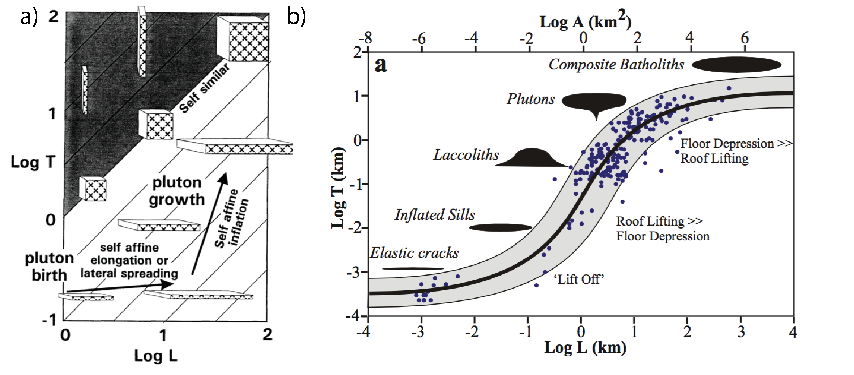
\includegraphics[scale=0.95]{Model.pdf}
    \caption{a) Schéma de  la formation des laccolites  en deux étapes
      par  \citet{McCaffrey:1997ea}.  Épaisseurs  en fonction  de leur
      longueur   de  différents   types  d'intrusions   magmatiques  à
      différentes locations.  Figure extraite de \citet{Cruden:tg}.}
    \label{C1-Model}
  \end{center}
\end{figure}

Les laccolites répertoriées par  \citet{E:2015tl} montrent un exposant
$a<1$  ($0.88 \pm  0.1$),  interprété comme  reflétant l'étalement  de
l'intrusion sur une  certaine distance sous forme d'un  sill avant son
épaississement (Figure \ref{C1-Model}). Ce modèle est cohérent avec le
modèle en  deux étapes couramment  accepté pour  la mise en  place des
laccolites \citep{Johnson:1973ho,McCaffrey:1997ea}.   Premièrement, le
magma s'étale latéralement au niveau de sa zone de flottabilité neutre
,  i.e.  $a<1$  jusqu'à  ce  qu'un sill,  caractérisé  par un  rapport
d'aspect assez large, soit formé.   Ensuite, lorsque le sill est assez
large, il s'épaissit par flexion  des couches sus-jacentes pour former
un    laccolite    caractérisé    par     une    valeur    de    $a>1$
\citep{Johnson:1973ho,Koch:1981if}.   Si  la   roche  sus-jacente  est
soumise à des contraintes trop  importantes, des failles se forment au
niveau des bords du sill et celui-ci s'épaissit uniformément sur toute
sa surface formant un  bysmalite \citep{E:2015tl}.  Dans la continuité
de  l'étude  de  \citet{McCaffrey:1997ea},  \citet{Rocchi:2002jy}  ont
réalisé une  étude détaillée du  complexe intrusif de l'île  d'Elbe en
Italie  et  ont trouvé  un  exposant  $a$  supérieur à  l'unité,  i.e.
$\sim  1.5$, interprété  comme étant  la preuve  de l'existence  d'une
phase dominée  par l'épaississement de l'intrusion  dans la croissance
de ces laccolites.

Des modèles plus récents conçoivent plutôt la formation des laccolites
par empilements successifs de sills, de grand rapport d'aspect, plutôt
que par  l'injection d'un seul volume  de magma fini à  un temps donné
\citep{Menand:2011ki}.   En effet,  ces  modèles sont  étayés par  les
expériences de \citet{Kavanagh:2006ig} (Section \ref{C1-sec:stockage})
où il  est montré  qu'un sill  peut se mettre  en place  à l'interface
entre deux couches  de rigidité différentes, la rigidité  de la couche
sus-jacente   étant   plus  importante   que   celle   de  la   couche
sous-jacente. Dès lors, la mise  en place d'un sill, en refroidissant,
procure un  environnement favorable  à la mise  en place  d'un nouveau
sill, soit au-dessus si la rigidité du sill solidifié est inférieure à
celle  de  la   roche  sus-jacente,  soit  en  dessous   dans  le  cas
contraire. Ce modèle de croissance a aussi été suggéré par de récentes
études  structurales  et  stratigraphiques, notamment  au  niveau  des
intrusions  de   tailles  intermédiaires  dans  les   Henry  Mountains
\citep{Horsman:2005ct,Morgan:2008hj,Horsman:2009gea,Menand:2011ki}. Ce
modèle, à  la différence  des modèles statiques  exposés plus  haut, a
aussi l'avantage de  pouvoir expliquer la structure  aplatie au niveau
du centre de certains laccolites \citep{Morgan:2008hj}.  Cependant, ce
modèle ne fournit pas de  mécanisme ni ne permet d'expliquer l'origine
de  la  loi  de  puissance  caractéristique de  la  géométrie  de  ces
intrusions. De plus, il ne permet pas de relier la géométrie finale de
l'intrusion  aux propriétés  physiques de  l'écoulement (volume,  taux
d'injection).

\citet{Nachwuchskoechin:2002tv}  ont réuni  des  données  sur une  plus
grande plage  de longueurs, de  petits filons de quelques  dizaines de
mètres à  des batholites de  quelques centaines de  kilomètres (Figure
\ref{C1-Model})  et  proposent  que  l'épaisseur  en  fonction  de  la
longueur des intrusions magmatiques forme une distribution en forme de
sigmoïde (dans une  échelle logarithmique), avec une  pente maximum de
$1.5$  caractéristique  des  laccolites.  Cependant,  aucune  théorie
sous-jacente ne soutient  cette observation.  De plus,  les données de
\citet{Cruden:tg}  sur les  larges sills  mafiques contredisent  cette
affirmation (Figure \ref{C1-Dimension}).

\subsection{Discussion}
\label{C1-sec:conclusion}

Bien que de  nombreux modèles ont été proposés pour  essayer de rendre
compte des observations, peu d'entre  eux s'intéressent à la dynamique
de l'intrusion qui  permettrait cependant de relier  la morphologie de
ces  intrusions aux  propriétés physiques  de l'écoulement  (volume ou
taux d'injection).   Afin de comprendre la  morphologie des intrusions
peu  profondes,  il  apparaît  donc important  de  s'intéresser  à  la
dynamique d'un tel écoulement.

\citet{Michaut:2011kg}   a  ainsi   développé   un  modèle   théorique
d'étalement d'un magma visqueux  sous une couche élastique d'épaisseur
contante  continuellement  nourrie  par  un conduit  vertical  en  son
centre.   Ce modèle  diffère de  ces prédécesseurs  par sa  capacité à
traiter la dynamique  même de l'intrusion ainsi que le  poids du magma
comme un  moteur de l'écoulement. Les  résultats et la capacité  de ce
modèle à  reproduire les observations  sont discutés dans  le chapitre
suivant.

\newpage
\bibliographystyle{agufull08}
\bibliography{/Users/thorey/Dropbox/Library}

%%% Local Variables:
%%% mode: latex
%%% TeX-master: "../main"
%%% End:
